\section{Introduction}

Artists often utilize real motion reference in the process of creating an animation to understand the key to successfully deliver certain actions and poses by working through the gathered examples. Even for highly exaggerated stylistic motion, the essential body mechanics transpire through the animation. This touch of reality, learned from the study of real life movements is essential to animate a believable movement. As the word implies, however, a reference is simply a starting point. The poses and timing information obtained from the reference will require most of the times the introduction of significant alterations in order to increase the appeal of the animation or fix the parts that did not translate well into the animation. Nonetheless, the little touch of reality insufflated into the animation through the reference strengthens the animation and reinforces its believability. Therefore, it would only seem natural to use motion data directly as a starting point of the animation process.

Despite these benefits, it is often considered difficult to apply motion data in keyframe animation pipeline because common methods of manipulating motion data are different from the process of production. Common methods typically edit the joint directly or rely on advanced motion editing techniques such as motion warping\cite{witkin1995motion} or motion stylization\cite{hsu2005style}. However, these methods are difficult to apply to animation pipeline because artists are trained to create character motion by character rig.
Rig, a control structure that allows to produce the motion of a 3D character, plays a key role in the animation production pipeline. A well-designed rig understands how an artist interacts with a character, provides an easy and efficient solution to produce complex motion,  and increases the productivity in animation generation\cite{mclaughlin2011character,orvalho2012facial}. Therefore, it would be an attractive idea to manipulate motion data with an artist-friendly rig. In this paper, we propose a novel mapping method from motion data to a general character rig. Our method can be seamlessly applied to the current animation production pipeline, and improve the efficiency in creating animation contents by directly mapping the existing motion data into parameters of character rig.

\begin{figure}[ht]
  \centering
  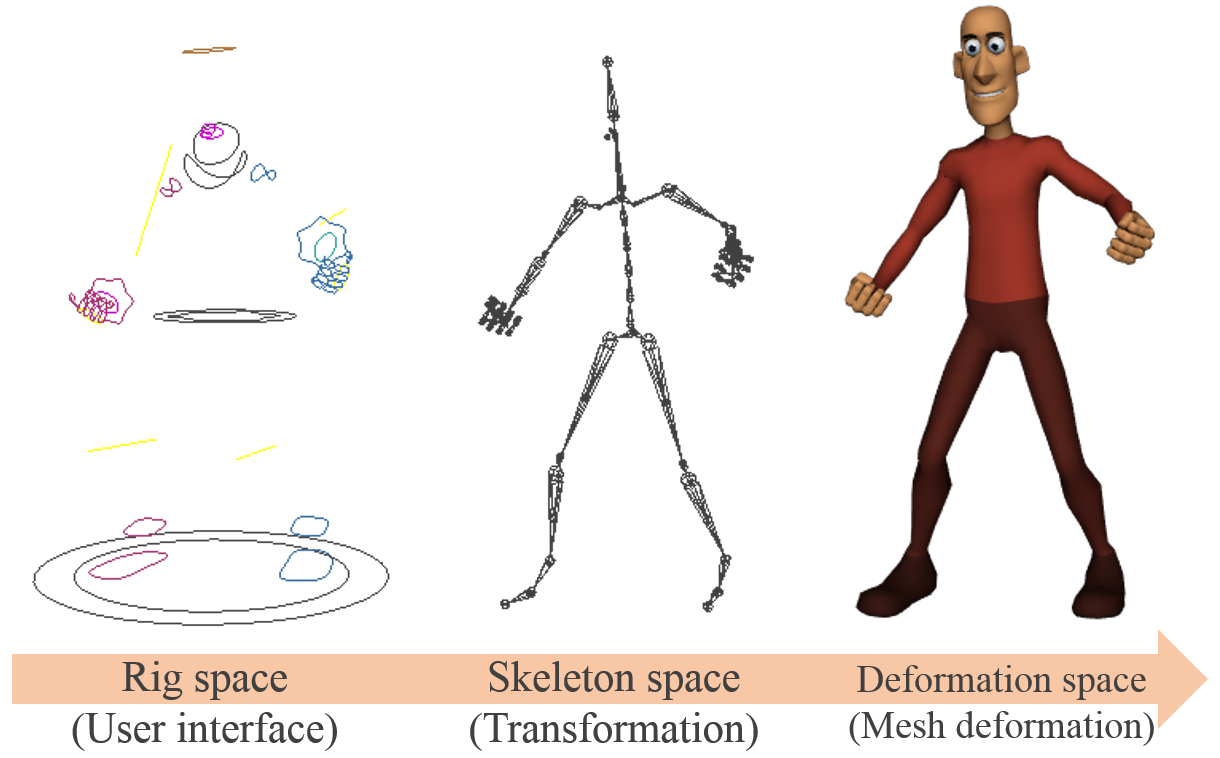
\includegraphics[width=1.0\linewidth]{images/rigLayer}
  \caption{Three layers of a character rig. The user interface layer controls the transformation layer, and the transformation layer in turn controls the skin deformer layer.}
  \label{fig:rigLayer}
\end{figure}

A character rig is composed of three layers\cite{orvalho2012facial} as shown in Figure \ref{fig:rigLayer}. The rig space, which is the user interface layer provides the artist with an interface that can control the skeleton space. In the skeleton space, the pose of a character is determined through the rigid body transformations applied to the hierarchical skeleton. Finally, the deformation layer deforms the character body by considering the correlation between the skeleton and the mesh vertices. Because our motion mapping occurs between the skeleton space and the rig space, we will not focus on the deformation layer in this study.

Artists are familiar with the rig space parameters and manipulate them skillfully for creation or editing of animation. However, this also means that the determination of the rig space depends on various factors such as the work preference of a specific artist, a desired rigging style, and the structure of a given character. Therefore, it is difficult to generally describe how the pose of a character can be represented in some optimal way, leading to multiple solutions for a single pose. Although such flexibility can help artists select preferred rig parameters depending on the task, it can cause ambiguity in the mapping process. 

Due to the aforementioned difficulties, professional artists often rely on manual identification of correlated operations between the skeleton space and the rig space in order to map motion data into the rig space parameters\cite{palamar2013mastering,DigitalTutor2013}. However, this approach suffers from a couple of drawbacks. First, as the mapping is performed on the positions and the orientations of the rig controllers, it is not clear how to handle user defined rig parameters that are often responsible for the generation of complex motions. Second, the manual process has to be repeated for a new character rig, making the process not well-scalable for a large scale production. Recently, Holden et al.\shortcite{holden2015learning} proposed an inverse rig mapping method based on a regression model, which incorporates example keyframe motion data prepared by an artist. Although this method works well with proper examples, it is often laborious to generate perfect example animations per each rig type.
%and the result of the inverse mapping can be biased toward the provided example data.

We propose an optimization-based inverse motion mapping method that does not rely on any manual specification of correspondences or prior data. Our inverse mapping problem finds the optimal rig parameters that minimize the distance between the pose generated by the rig parameters and the pose of the input motion. We first perform the rig analysis process that automatically groups the skeleton and the rig parameters, where each group has mutually independent rig operations with each other. Based on these groups, we divide the problem into a set of sub-problems and efficiently perform the optimization.

We also propose a novel skeletal representation on the $SE(3)$ Lie group manifold to measure the distance accurately between the poses during the optimization process. Mathematically, rigid body rotations or translations are members of the special Euclidean group $SE(3)$\cite{murray1994mathematical}, and therefore, the skeletal pose with multiple rigid body segments can be expressed as a point on the Lie group \SE. Geometrically, the Lie group \SE{} is a curved manifold, and therefore, the measure of the distance between two poses corresponds to the geodesic distance of the two points on the manifold. To overcome the difficulty of directly minimizing the geodesic distance, we linearize the Lie group \SE{} motion into the vector space which is the Lie algebra \se{}. We then perform our optimization as a linear programming.

During the optimization stage, we solve the ambiguity arising in the mapping process by regularizing the rig parameters. An artist who utilizes the rig would choose the most efficient rig parameters for a given animation task, based on his/her experiences and skills. This implies that the optimality of the rigging depends on the working style of the individual animator. However, a rigger who creates the rig would prefer a solution that results in minimum differences of sparse rig parameters. We opt to perform the regularization of the rig parameters to obtain sparse solutions. In addition, we allow the artist to additionally specify constraints on the rig parameters, to make the parameters converge toward the direction that complies with the artist's intention. This can solve errors frequently occurring in the motion mapping process such as self-penetration. We demonstrate the efficiency and usability of our method by performing the mapping onto various rigs and also show how seamlessly our approach can be applied to the production pipeline.




%\subsection{prev}
%Rig, which is defined as a control method to produce the motion of  a 3D character[V.Orvalho,2010], plays a key role in the animation production pipeline. Well designed rig understands how an artist interacts with a character, provides an easy and efficient solution to produce complex motion and thus, improve the productivity in animation generation\cite{mclaughlin2011character}.
%
%In this paper, we propose a novel inverse mapping method from motion data to general character rig.
%Our method can be seamlessly applied to current animation production pipeline, and improve the efficiency (in motion generation and editing) by directly mapping the existing motion data into parameters of character rig.
%Due to the effectiveness, the idea of using rig with motion data got attention in real production too.
%
%Character rig has 3 levels of data flow structure as shown in Figure \ref{fig:rigLayer}\cite{orvalho2012facial}. The top level called user interface layer provides an animator the interface which can control the transform layer. The transform layer decides the character pose through the rigid body transformation of hierarchical skeleton.
%Finally, the deformation layer shows character animation by deforming the character body considering the correlation between the skeleton and mesh vertices. 
%
%Here, we define the rig space as the user interface layer which is composed of various rig parameters that are controlled by the animator to produce character motion.
%The motion data is represented in skelton space, which is defined as skeleton parameters in transform layer. Since the inverse motion mapping problem is held in the skeleton space and the rig space, we are not going to handle the deformation layer directly.
%
%From the fact that the rig space parameters are directly used by artist(animator), it is important(valuable) and useful space for editing and modifying process in real animation production.
%
%However, the rig space is an abstract space. The direct interaction with an artist makes rig space dependent on character structure, work preference of animator, and rigging style of rigger, and thus, it is difficult to generally describe how rig space parameters decide the character pose.
%
%Due to the difficulties described above, a general approach of mapping motion data into rig space parameters is manually defining the correlation between the skeleton space and the rig space.[Maya][Animbinder][DigitalTutor]
%However, this requires a repetitive manual process on new rig, and only the simple mapping that uses the position and the orientation constraint is applicable.
%Therefore, this approach is not proper for production nor valid for user defined rig parameters that generates complex motion.
%Recently, \cite{holden2015learning} proposed the inverse mapping method of rig space parameters that does not require manual correspondence by using the example animation generated by animators.
%However, it is still laborious to generate example animation per each rig type, and the result of inverse mapping is biased to the example data.
%Our method does not require any manual correspondence, or prior data.
%
%The inverse mapping problem can be defined as finding the optimal rig parameter $R$ that minimize the distance between pose $P(R)$ which is generated by $R$ and input motion pose $P$.
%We first perform the rig analysis process that automatically generates correlation map between $P$ and $R$ without any prior.
%Then, we group the parameters that has correlation to each other.
%Since rig operation of each group is independent, we can divide the problem into list of sub-problem and efficiently perform the optimization.
%
%To measure the accurate distance between $P$ and $P(R)$, instead of using joint position or angle based representation, we propose a novel skeletal representation. 
%
%Mathematically(Theoretically), all rigid body rotation and translation is a member of special Euclidean group $SE(3)$ in a Lie group[ref?], and therefore, the skeletal pose generated by rig can be expressed as a point on the Lie Group $SE(3) \times …  \times SE(3)$(Figure 3). 
%
%Geometrically, the Lie group $SE(3) \times ... \times SE(3)$ is a curved manifold which makes our measurement of distance between $P$ and $P(R)$ into the geodesic distance of two points on the curved manifold. Since it is difficult to directly minimze the distance on it, we linearized the Lie group $SE(3) \times ... \times SE(3)$ motion into the vector space or Lie algebra $se(3) \times ... \times se(3)$ and efficiently sovled the problem.
%
%Generally, rig is designed to provide multiple solutions for a single pose (to make flexible user interface). Therefore, $P$ and $R$ is not one-to-one correspondence.
%The solution to ambiguity in mapping problem is selecting the most optimal rig.
%
%From the artist point of view, the optimality depends on artist style, work environment resulting the problem ambiguous.
%However, from the rigger (character technical director) and rig’s functionality point of view, we can define the optimality.
%Based on this, we performed the regularization for rig parameters.
%In the results section, we show our regularized rig parameters are also efficient for artists too.
%
%Finally, by letting the animator to assign(add) the constraints in rig parameters, it converge as what animator intended.
%This can solve the error that is frequently shown in motion mapping process such as self penetration.
%In the results section, we show the efficiency and usability of our method by performing on various rig and seamlessly applying to real production pipeline.
%


%%%%% deprecated sentences

%Recent trend shows that using the rig with motion data can even increase the produc
%Recently, using rig with motion data got attention in real production. [ref?]

%Recently, the mapping method of the motion capture or keyframe motion data into the rig space got attention in (real) production.

%The virtue of this method is that the existing motion data can be seamlessly applied to animation pipeline, and consequently, improves the efficiency in animation production.
%However, unlike other layers, a direct interaction with artists makes the rig space an abstract space.
%Since the rig space provides user interface depending on the structure of character, work preference of animator, and rigging style of rigger, it is difficult to generally describe how rig space parameters decide the character pose.

%The mapping method of the motion capture or keyframe motion data into the rig space enable existing data reproducable.
%To use rig with the motion data, the motion data must be first mapped into rig space parameters.
%Due to the difficulties described above, a general approach is manually defining the relationship between the skeleton space and the rig space.[Maya][Animbinder][DigitalTutor]

%We used a rig space motion optimization to solve the inverse mapping problem of robust skeleton motion to general rig space without any manual correspondence or example motion data.

%The skeleton space is represented as hierarchical rigid body skeleton’s transformation.
%Even if rig has squash and stretch parameter, we can represent it with rigid skeleton’s translation without changing the skeleton length.

%Geometrically, our measurement is geodesic distance between $p$ and $P(R)$, which are two points on a Lie group $SE(3) \times ... \times SE(3)$.
%However, a Lie group $SE(3) \times ... \times SE(3)$ is a curved manifold which is difficult to directly minimize thd distance. Therefore, we linearized $SE(3) \times ... \times SE(3)$ motion into vector space Lie algebra $se(3) \times ... \times se(3)$ and efficiently sovled the problem.
%Geometrically, a Lie group $SE(3) \times ... \times SE(3)$ is a curved manifold, and our measurement which is the distance between $P$ and $P(R)$ on Lie group is defined as geodesic distance.
%However, it is difficult to directly minimize the distance. We overcome(solve) the issue by linearizing $SE(3) \times ... \times SE(3)$ motion into vector space Lie algebra $se(3) \times ... \times se(3)$.

%we define the "priority" in rig parameter from the rigger and rig functionality point of view.

%Since there is no prior knowledge, we cannot provide the unique optimal solution which satisfies the preferences of individual artist.
